\documentclass[12pt]{article}

\usepackage{amsfonts, amsmath, amssymb, amsthm, dsfont, enumitem, fancyhdr, graphicx, mathtools}
%\usepackage{tikz-cd}
\usepackage[margin=1in, includehead, includefoot, heightrounded]{geometry}
\allowdisplaybreaks
\pagestyle{fancy}
\rhead{Erick Lin}

\newcommand{\norm}[1]{\left\lVert#1\right\rVert}
\newcommand*\dist{\mathop{\!\mathrm{d}}}
\DeclareMathOperator{\im}{Im}
%\let\ker\relax %RedeclareMathOperator
%\DeclareMathOperator{\ker}{Ker}
\DeclareMathOperator{\Hom}{Hom}
\DeclareMathOperator{\Ext}{Ext}
\renewcommand{\thesubsection}{\arabic{subsection}}
\newcommand{\inc}{\xhookrightarrow{}}
\newcommand*\sq{\mathbin{\vcenter{\hbox{\rule{.4ex}{.4ex}}}}}
\newcommand{\iso}{\approx}
\newcommand{\RP}{\mathbb{R}\mathrm{P}}
\newtheorem{theorem}{Theorem}
\newtheorem{lemma}[theorem]{Lemma}

\begin{document}

\section*{MATH 6441 -- HW9 Solutions}
\subsection*{Section 3.2}
%http://www.math.brown.edu/~tomg/hw2comments.pdf
%http://math.ucr.edu/~res/math205B-2012/helpfile.pdf
\begin{enumerate}
    \item[1.]
        \boldmath\textbf{Assuming as known the cup product structure on the torus $S^1 \times S^1$, compute the cup product structure in $H^*(M_g)$ for $M_g$, the closed orientable surface of genus $g$, by using the quotient map from $M_g$ to a wedge sum of $g$ tori, shown below.
        }\unboldmath \par
        {\centering
            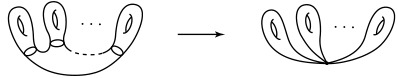
\includegraphics[scale=1]{Mg_quotient}
        \\}
        %From Example 2.36, we know that $H_0(M_g) = H_2(M_g) = \mathbb{Z}$ and $H_1(M_g) = \mathbb{Z}^{2g}$. \par
        The cohomology of $S^1 \times S^1$ has a basis consisting of $\alpha, \beta \in H^1$ and $\gamma \in H^2$ satisfying $\alpha \smile \alpha = 0$, $\beta \smile \alpha = -\gamma$, and $\beta \smile \beta = 0$. To find the cohomology of the quotient $M_g / A$, which is a wedge sum of $g$ tori, we first show how the cup product structure can be composed under the wedge sum in general. If $X = \bigvee_{i = 1}^n X_i$ where the $X_i$ are CW complexes, then the inclusions $X_i \inc X$ together induce an isomorphism $H^*(X) \to \prod_{i = 1}^n H^*(X_i)$, whose inverse is (by excision) induced by the retractions $X \to X_i$. Because the induced maps $H^*(X_i) \to H^*(X)$ and $H^*(X) \to H^*(X_i)$ are ring homomorphisms (determining the cup product of elements from the same $H^*(X_i)$), they together give a ring isomorphism $H^*(X) \to \prod_{i = 1}^n H^*(X_i)$, so the cup product of elements from $H^*(X_i)$ and $H^*(X_j)$ for $i \neq j$ is zero. Thus, the cohomology of $M_g/A$ has a basis consisting of $\alpha_i, \beta_i \in H^1$ and $\gamma_i \in H^2$ satisfying $\alpha_i \smile \beta_i = \gamma_i$, $\beta_i \smile \alpha_i = -\gamma_i$, and all other cup products equal to zero for all $1 \leq i \leq g$. \par
        Because the homology of $A$ is given by $H_1$ and the map $H_1(A) \to H_1(M_g)$ is zero, the quotient map $M_g \to M_g/A$ induces an isomorphism in $H_1$ and an injection in $H_2$, and so it induces an isomorphism in $H^1$ and a surjection in $H^2$. We also have that the generators $\gamma_i$ of the basis of $H^2(M_g/A)$ all map to the same generator $\gamma$ of $H^2(M_g)$. Thus, the cohomology of $M_g$ is the same as the cohomology of $M_g/A$ except that all the $\gamma_i$ are replaced by a single $\gamma$.

    \item[7.]
        \boldmath\textbf{Use cup products to show that $\RP^3$ is not homotopy equivalent to $\RP^2 \vee S^3$.
        }\unboldmath \par
        We know that the inclusion $S^3 \inc \RP^2 \vee S^3$ induces an isomorphism in $H^3(\RP^2 \vee S^3; \mathbb{Z}/2)$ and the trivial map in $H^1(\RP^2 \vee S^3; \mathbb{Z}/2)$, so the third power of every generator is zero. On the other hand, we can find a generator of $H^1(\RP^2; \mathbb{Z}/2)$ whose third power is nonzero.

    \item[11.]
        \boldmath\textbf{Using cup products, show that every map $S^{k + l} \to S^k \times S^l$ induces the trivial homomorphism $H_{k + l}(S^{k + l}) \to H_{k + l}(S^k \times S^l)$, assuming $k > 0$ and $l > 0$.
        }\unboldmath \par
        A generator of $H^{k + l}(S^k \times S^l)$ is a product $a \smile b$ where $a \in H^k(S^k \times S^l)$ and $b \in H^l(S^k \times S^l)$. Then for any map $f : S^{k + l} \to S^k \times S^l$, the induced map $f^* : H^{k + l}(S^{k + l}) \to H^{k + l}(S^k \times S^l)$ satisfies $f^*(a \smile b) = f^*(a) \smile f^*(b) = 0$ since $f^*(a) \in H^k(S^k \times S^l) = 0$. Dualizing shows that in this case, the induced map $H_{k + l}(S^{k + l}) \to H_{k + l}(S^k \times S^l)$ is trivial as well.
\end{enumerate}
\end{document}
